\documentclass{article}

\usepackage{graphicx}
\usepackage{mathtools}
\DeclarePairedDelimiter{\ceil}{\lceil}{\rceil}

\graphicspath{ {./images/} }

\begin{document}
\section{Data}
The problem instances used in the paper are networks classified by the number of edges, a M, and the number of nodes, b, and labelled MaNb accordingly. An example of these networks can be seen in figure \ref{fig:netExamples}. Additionally, the probability that the target is on a given edge is either uniformly distributed or non-uniformly distributed. The paper describes a specific way that the non-uniform distribution is defined, described in section \ref{Prob}.
\begin{figure}[h]
    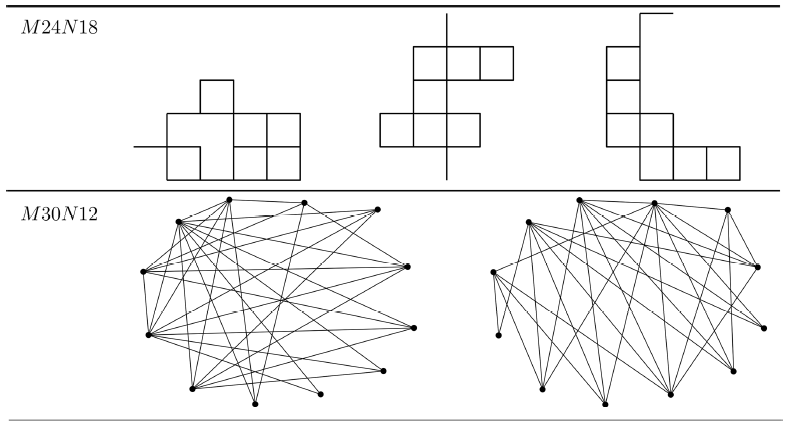
\includegraphics[width=\textwidth]{networkExamples}
    \caption{Example networks from the paper}
    \label{fig:netExamples}
\end{figure}

\section{Problem Generation}
The paper describes two methods that are used to generate the networks based on the ratio of edges to nodes. If the ratio is smaller than 2, a sparse graph is generated, amd if this ratio is greater than or equal to 2, a dense graph is generated.
\subsection{Probabilities} \label{Prob}
The two types of probability distributions for a target on a given graph can either be uniform or non-uniform. The uniform distribution means each edge has a probability of \[\frac{1}{M}\] where M is the number of edges in the graph.
The non-uniform probability is more complicated. Edges in the graph are randomly chosen to be low, medium or high probability. The number of each of these edges is in proportion low:medium:high $\approx$ 1:2:1, such that the sum of low, medium and high edges = M (the number of edges in the graph). Each of these edges is assigned a probability that is low, medium or high in a ratio of $p_{low}$:$p_{medium}$:$p_{high}$ $\approx$ 1:2:3. Note that the sum of the probability for all edges must equal 1 (within some sufficiently small epsilon)

\subsection{Dense Graphs}
Dense graphs are generated by creating N nodes, then randomly connecting them with M edges. It is necessary to check that the graph is connected after generation, but otherwise, the generation is quick and easy.

\begin{figure}[h]
    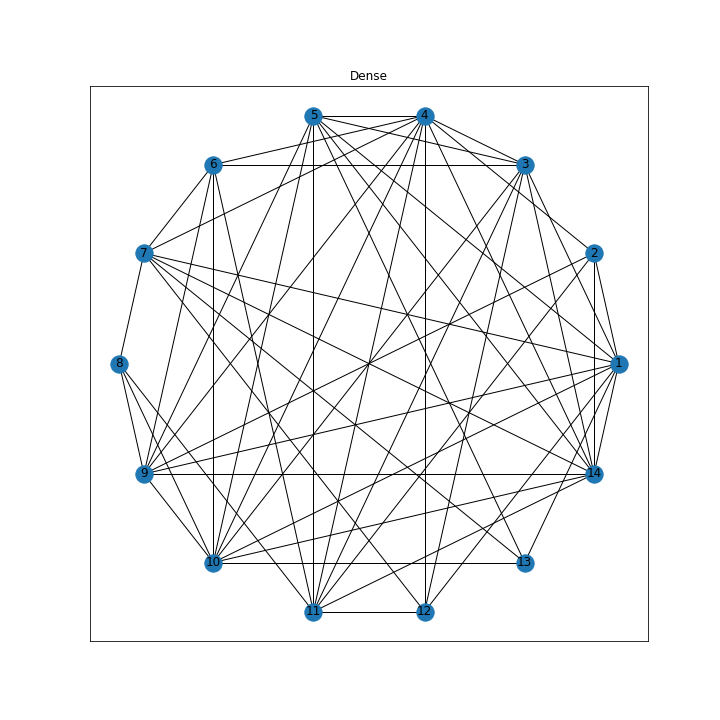
\includegraphics[width=\textwidth]{dense}
    \caption{An M50N14 dense graph}
    \label{fig:dense}
\end{figure}

An example dense graph is seen in figure \ref{fig:dense}.

\newpage
\subsection{Sparse Graphs}
Sparse graphs are generated in a grid-like structure that simulates a manhattan city block. First, a random spanning tree with N nodes and N-1 edges is made on a 10x10 grid. Then, edges from the grid are added to connect nodes in the spanning tree until M edges are reached. This sounds relatively simple to do, however there were issues encountered while generating the tree. 
Originally a spanning tree was created in the grid using a breadth first search, but this was not a random tree, so the results were near complete grids, instead of grids with holes in them like the example sparse networks in the paper. The method was adjusted to add a random number of neighbouring nodes for each node in the tree while it was generated. This made the graphs more similar to the examples in the paper, and provided more interesting problem instances. 

However, other problems ocurred when there were not enough available places to add an edge without creating new nodes. This was problematic because if new nodes were added, the graph would be the incorrect class, but without being able to add the edges, the graph would be the incorrect class anyway. This was worked around by simply generating a new instance of the graph class, although methods for removing leaf nodes from the graph and repositioning them to produce more potential edge places were considered, but not competely implemented.
\begin{figure}[h]
    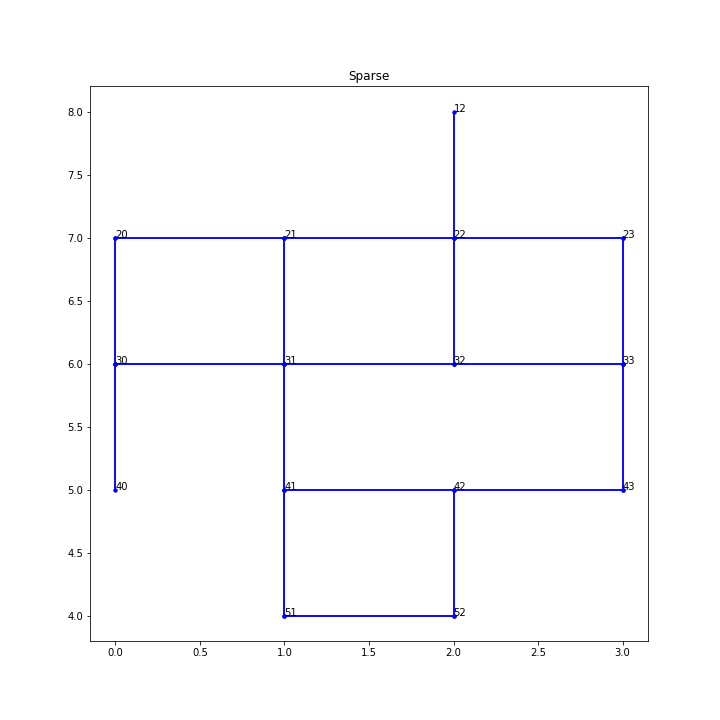
\includegraphics[width=\textwidth]{sparse}
    \caption{An M19N15 sparse graph}
    \label{fig:sparse}
\end{figure}

An example sparse graph is seen in figure \ref{fig:sparse}.


\subsection{Improvements and Extensions}
Improvements were made to the problem generation so that it was easier to generate instances of varying sizes, and so that errors in instances were reduced. Improvements include defining a better threshold for when to generate a sparse or dense graph, and making a visualisation tool for search strategies, so that the optimal strategy can be shown on any given graph. 
The tighter threshold was defined to help ensure valid graphs can be made. For example, on a 10 x 10 grid, the maximum number of nodes possible for a sparse graph is 100, and the maximum number of edges possible is 180. The ratio between these values is 1.8 which is less than 2, so a sparse graph is generated. However, if 181 edges are chosen with 100 nodes, the ratio is 1.81, also less then 2 so a sparse graph is chosen to be made. However, this is impossible because there are no more spaces to add an edges. This means a dense graph should be made because a sparse graph of the correct class cannot be generated.
 The threshold defined in the paper does not take this into account, and so ignores a range of graph classes. After creating the functionality for generating graphs, many classes were generated with different nodes to see if there was a pattern for when a closer threshold could be obtained. For a given number of nodes, the number of edges in a valid sparse graph, and valid dense graph were noted, and then formulae for these numbers in terms of nodes were created. The table is shown below.

 \begin{center}
    \begin{table}[h]
        % \footnotesize
        Valid Edges for graphs of n nodes\\
        \begin{tabular}{ |c|c|c| }
        \hline
        Nodes & Largest Valid Edges - Sparse  & Largest Valid Edges - Dense\\
        \hline
        1 & 0 & 0 \\ \hline
        2 & 1 & 1 \\ \hline
        3 & 2 & 3 \\ \hline
        4 & 4 & 6 \\ \hline
        5 & 5 & 10 \\ \hline
        6 & 7 & 15\\ \hline
        7 & 8 & 21 \\ \hline
        8 & 10 & 28 \\ \hline
        9 & 12 & 36 \\ \hline
        \end{tabular}
    \end{table}
    \end{center}

    This table outlines the largest number of edges that can be used to make a sparse and dense graph with the given number of nodes. Since there is no upper bound on the number of edges for dense graphs, it is clear that the maximum number of edges for a dense graph with $n$ nodes is $\binom{n}{2}$, corresponding to the complete graph $K_n$. The pattern for the sparse graph was less obvious. Due to the grid structure of the sparse networks, the number of new edges that can be added when a new node is added changes based on if the node will complete a square in the grid. It turns out that this sequence is the number of edges in a spiral of $n$ unit squares. The formula for the nth term in the sequence is $a(n) = 2n - \lceil 2\sqrt{n} \rceil$.This was found by searching the Online Encyclopedia of Integer Sequences (OEIS) REFERENCE HERE. This formula is important as it provides a tighter threshold condition for when to generate a sparse or dense graph. That is, if $a \geq 2b - \lceil 2\sqrt{b} \rceil$ where a is the number of edges and b is the number of nodes in the graph, then the graph is dense, otherwise it is sparse.
\section{Results}
\subsection{Result Visualisation}
A tool was developed to help visualise the optimal search strategy for a given graph. Unvisited edges are indicated in blue, visited edges are indicated in green, and edges that are being visited in the current time slot t, are red.
\begin{table}
% \footnotesize
M19N15\\
\begin{tabular}{ |c|c|c|c|c|c|c|c|c|c|c|c|  }
\hline
Scenario & 1 & 2 & 3 & 4 & 5 & 6 & 7 & 8 & 9 & 10 & Average\\
\hline
K1-Uniform & 10.5 & 10.026 & 9.711 & 10.079 & 10.395 & 9.974 & 10.026 & 9.816 & 10.026 & 10.237 10.079\\ \hline
K1-Non-Uniform & 9.421 & 8.5 & 8.658 & 8.368 & 9.5 & 8.553 & 9.263 & 8.5 & 9.0 & 8.737 8.85\\ \hline
K2-Uniform & 5.026 & 4.868 & 4.816 & 4.763 & 5.079 & 4.816 & 4.974 & 4.763 & 4.868 & 5.026 4.9\\ \hline
K2-Non-Uniform & 4.5 & 4.158 & 4.211 & 4.132 & 4.5 & 4.184 & 4.184 & 4.0 & 4.421 & 4.342 4.263\\ \hline
\end{tabular}
\end{table}

\begin{table}
% \footnotesize
M19N15\\
\begin{tabular}{ |c|c|c|c|c|c|c|c|c|c|c|c| }
\hline
Scenario & 1 & 2 & 3 & 4 & 5 & 6 & 7 & 8 & 9 & 10 & Average\\
\hline
K1-Uniform & 225.886 & 133.58 & 10.016 & 81.72 & 502.555 & 311.777 & 286.554 & 18.267 & 25.862 & 353.577 194.98\\ \hline
K1-Non-Uniform & 58.818 & 6.563 & 15.017 & 3.781 & 44.877 & 10.219 & 63.205 & 8.016 & 13.36 & 6.141 23.0\\ \hline
K2-Uniform & 16.027 & 8.579 & 0.609 & 0.75 & 53.019 & 2.219 & 12.235 & 2.828 & 5.5 & 16.471 11.824\\ \hline
K2-Non-Uniform & 1.831 & 0.562 & 1.188 & 0.75 & 1.422 & 1.0 & 0.578 & 0.156 & 4.86 & 1.828 1.418\\ \hline
\end{tabular}
\end{table}

\begin{table}
% \footnotesize
M19N15\\
\begin{tabular}{ |c|c|c|c|c|c|c|c|c|c|c|c }
\hline
Scenario & 1 & 2 & 3 & 4 & 5 & 6 & 7 & 8 & 9 & 10 & Average\\
\hline
K1-Uniform & 0.0 & 0.0 & 0.0 & 0.0 & 0.0 & 0.0 & 0.0 & 0.0 & 0.0 & 0.0 0.0\\ \hline
K1-Non-Uniform & 0.0 & 0.0 & 0.0 & 0.0 & 0.0 & 0.0 & 0.0 & 0.0 & 0.0 & 0.0 0.0\\ \hline
K2-Uniform & 0.0 & 0.0 & 0.0 & 0.0 & 0.0 & 0.0 & 0.0 & 0.0 & 0.0 & 0.0 0.0\\ \hline
K2-Non-Uniform & 0.0 & 0.0 & 0.0 & 0.0 & 0.0 & 0.0 & 0.0 & 0.0 & 0.0 & 0.0 0.0\\ \hline
\end{tabular}
\end{table}
\end{document}